\documentclass{beamer}

% % % % % % % % % % % % % % % % % % % % 
% Preblem
%
\usetheme{metropolis}
\usepackage[backend=bibtex,style=authoryear]{biblatex}
\addbibresource{references.bib}

% add commar between name and year \ Default (Name Year), Renew (Name, Year)
\renewcommand*{\nameyeardelim}{\addcomma\addspace}

% - - - - - - - - - - - - - - - - - - - -
% NEED BY \makethesiscover
% - - - - - - - - - - - - - - - - - - - -
% Common
\newcommand{\studentEmailaddress}{sitdhibong.l@student.chula.ac.th}
% English letters
\newcommand{\ThesisNameEN}{Test Case Generation from a Java Static Call Graph}
\newcommand{\authorNameEN}{Sitdhibong Laokok}
\newcommand{\prefixEN}{Mr.}
\newcommand{\studentnameEn}{{\prefixEN}~{\authorNameEN}}
\newcommand{\curriculumnEn}{Master of Science}
\newcommand{\majorEn}{Software Engineering}
\newcommand{\departmentEn}{Computer Engineering}
\newcommand{\facultyEn}{Faculty of Engineering}
\newcommand{\universityEn}{Chulalongkorn University}
\newcommand{\disclaiminationEn}{Copyright Year 2016}
\newcommand{\advisorEn}{Assoc. Prof. Taratip Suwannasart, Ph.D.}
\newcommand{\engkeywords}{Test case generation, Java language, Static call graph}
\newcommand{\academicYearEn}{2016}


\usepackage[font=scriptsize]{caption}
\usepackage{mwe}

\definecolor{brewcolorRed}{RGB}{150,4,12}

\setbeamercolor{frametitle}{fg=white,bg=brewcolorRed}

\metroset{%
    progressbar=head
}

\useinnertheme{rectangles}

\defbeamertemplate*{footline}{}%
{
    \leavevmode%
    \hbox{%
        \begin{beamercolorbox}[wd=.3\paperwidth,ht=2ex,dp=2ex,center]{section in footer}%
            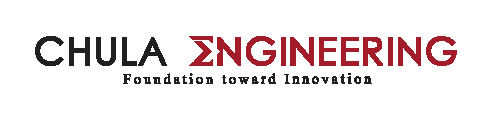
\includegraphics[width=0.25\paperwidth]{figure/chula-engineering}
        \end{beamercolorbox}

        \begin{beamercolorbox}[wd=.5\paperwidth,ht=2ex,dp=2ex,center]{subsection in footer}%
            \insertsubsection
            \vspace{0.2cm}
        \end{beamercolorbox}

        \begin{beamercolorbox}[wd=.2\paperwidth,ht=6ex,dp=2ex,right]{pagenumber in footer}%
            \vfill
            \insertframenumber{}\hspace{1cm}
            \vspace{0.2cm}
        \end{beamercolorbox}
    }
}

% % % % % % % % % % % % % % % % % % % % 

% % % % % % % % % % % % % % % % % % % % 
% Title config
%
\title{\ThesisNameEN}
\subtitle{IMECS2017}
\date[2017.03.14]{\today}
\author{\authorNameEN~\small{and~\advisorEn}}
\institute{{\facultyEn}, {\universityEn}}
% % % % % % % % % % % % % % % % % % % % 

\begin{document}

\maketitle

\begin{frame}[t]
    \frametitle{Agenda}
    \tableofcontents[hideallsubsections]
\end{frame}

% % % % % % % % % % % % % % % % % % % % 
% Introduction
%
\section{Introduction}
\begin{frame}{Introduction}
  Hello
\end{frame}

\begin{frame}{Faults Detection Metric}
    \begin{figure}
        \begin{equation}
            APFD~=~1-~\frac{\sum^{num_f}_{i=1}{TF_i}}{{num}_t \cdot {num}_f} %
                    +~\frac{1}{2 \cdot {num}_t}
            \label{eq:apfd}
        \end{equation}
        \caption{Average Percentage Faults Detected metric \parencite{792604}}
        \label{fig:apfd}
    \end{figure}
\end{frame}
% % % % % % % % % % % % % % % % % % % % 

% % % % % % % % % % % % % % % % % % % % 
% Related works
%
\section{Related works}
% % % % % % % % % % % % % % % % % % % % 

% % % % % % % % % % % % % % % % % % % % 
% Background
%
\section{Background}
\subsection{Program graph}
\begin{frame}{Program graph}
    \begin{enumerate}
        \item Control Flow Graph
        \item Static Call Graph
    \end{enumerate}
\end{frame}

\begin{frame}{Control Flow Graph}
    \textbf{Control flow graph definition}
    \parencite{Allen:1970:CFA:390013.808479}
\end{frame}

\begin{frame}{Control Flow Graph}
    \begin{figure}
        
\includegraphics[width=0.7\paperwidth]{figure/Primitive-Operation-Structure.eps}
        \caption{Primitive operation structure \parencite{McCabe1976}}
        \label{fig:primitivestructure}
    \end{figure}
\end{frame}

\begin{frame}{Program graph}
    \begin{enumerate}
        \item<1-> Control Flow Graph
        \item<2-> Static Call Graph
    \end{enumerate}
\end{frame}

\begin{frame}{Static Call Graph}
    \textbf{Example}
\end{frame}

% % % % % % % % % % % % % % % % % % % % 

% % % % % % % % % % % % % % % % % % % % 
% Proposed approach
%
\section{Proposed Approach}
\subsection{Overview}
\begin{frame}{Methodology overview}
    \begin{figure}
        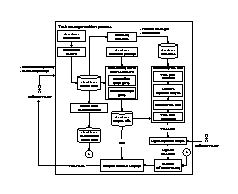
\includegraphics[height=0.65\paperheight]{figure/Methodology.eps}
        \caption{Methodology of Test Case Generation based on Static Data}
        \label{fig:methodologyOverview}
    \end{figure}
\end{frame}

\subsection{B. Constant collection}
% % % % % % % % % % % % % % % % % % % % 

% % % % % % % % % % % % % % % % % % % % 
% Conclusion
%
\section{Conclusion}
\begin{frame}{Conclusion}
    \begin{itemize}
        \item<1->aaaa
        \item<2->bbbb
        \item<3->cccc
    \end{itemize}
\end{frame}
% % % % % % % % % % % % % % % % % % % % 
\end{document}
